\begin{pastexam}[label={px:df3-103-ds-03}]{地方三等資訊處理 103 年 第三題}
（申論；15 分）

請用 Dijkstra 演算法找出下圖中從 S 到 T 的最短路徑長度：
\begin{itemize}[leftmargin=2.2em, nosep]
\item[㈠] 請依序寫出過程中逐一加入已被選擇的頂點（vertex），起始頂點為 S。（10 分）
\item[㈡] 請問以此演算法所找出的 S 到 T 最短路徑長度為何？（5 分）
\end{itemize}
\begin{center}
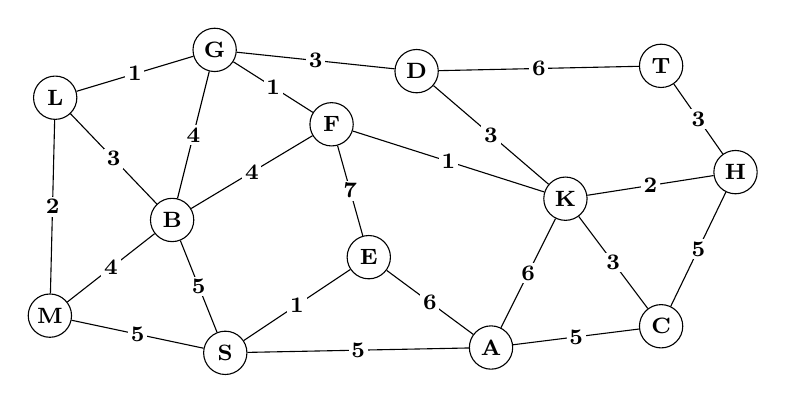
\begin{tikzpicture}[v/.style={circle,draw,minimum size=5.5mm,inner sep=0pt,font=\footnotesize\bfseries},
  lab/.style={font=\footnotesize\bfseries,fill=white,inner sep=1pt}, x=1.35cm, y=1.35cm]
\node[v] (L) at (0.5,-1.1) {L};
\node[v] (G) at (2.0,-0.65) {G};
\node[v] (D) at (3.9,-0.85) {D};
\node[v] (T) at (6.2,-0.8) {T};
\node[v] (F) at (3.1,-1.35) {F};
\node[v] (H) at (6.9,-1.8) {H};
\node[v] (B) at (1.6,-2.25) {B};
\node[v] (K) at (5.3,-2.05) {K};
\node[v] (E) at (3.45,-2.6) {E};
\node[v] (M) at (0.45,-3.15) {M};
\node[v] (C) at (6.2,-3.25) {C};
\node[v] (S) at (2.1,-3.5) {S};
\node[v] (A) at (4.6,-3.45) {A};
\draw (L) -- node[lab] {1} (G);
\draw (G) -- node[lab] {3} (D);
\draw (G) -- node[lab] {1} (F);
\draw (D) -- node[lab] {6} (T);
\draw (L) -- node[lab] {3} (B);
\draw (G) -- node[lab] {4} (B);
\draw (F) -- node[lab] {4} (B);
\draw (F) -- node[lab] {1} (K);
\draw (F) -- node[lab] {7} (E);
\draw (D) -- node[lab] {3} (K);
\draw (T) -- node[lab] {3} (H);
\draw (K) -- node[lab] {2} (H);
\draw (L) -- node[lab] {2} (M);
\draw (M) -- node[lab] {4} (B);
\draw (B) -- node[lab] {5} (S);
\draw (M) -- node[lab] {5} (S);
\draw (S) -- node[lab] {1} (E);
\draw (S) -- node[lab] {5} (A);
\draw (E) -- node[lab] {6} (A);
\draw (K) -- node[lab] {6} (A);
\draw (K) -- node[lab] {3} (C);
\draw (H) -- node[lab] {5} (C);
\draw (A) -- node[lab] {5} (C);
\end{tikzpicture}
\end{center}
\end{pastexam}

\begin{pastsoln}
答案：㈠ 依序選入 S、E、A、B、M、L、F、G、K、C、D、H、T。 ㈡ $14$（路徑 S--E--F--K--H--T）。

圖是無向圖，邊權都是正的，可以用 Dijkstra（資結書第~25.2~節、虛擬碼~25.3）。 每一步從還沒選的頂點中選
距離估計 $d$ 最小的加入，再用它鬆弛鄰居。 $d$ 相同時依字母順序選（選法不影響最後的距離）。

\textbf{追蹤}（每列是選入一個頂點之後更新的距離；沒列出的頂點維持原值或 $\infty$）：
\begin{center}
\small
\begin{tabular}{clll}
\toprule
步 & 選入（$d$） & 鬆弛後變小的距離 & 說明 \\
\midrule
1 & S (0) & B 5、M 5、E 1、A 5 & \\
2 & E (1) & F 8 & A：$1 + 6 = 7 > 5$ 不變 \\
3 & A (5) & K 11、C 10 & A、B、M 同為 $5$，依字母先選 A \\
4 & B (5) & L 8、G 9 & F：$5 + 4 = 9 > 8$ 不變 \\
5 & M (5) & L 7 & $5 + 2 = 7 < 8$ \\
6 & L (7) & G 8 & $7 + 1 = 8 < 9$ \\
7 & F (8) & K 9 & F、G 同為 $8$；K：$8 + 1 = 9 < 11$ \\
8 & G (8) & D 11 & \\
9 & K (9) & H 11 & D：$9 + 3 = 12 > 11$；C：$12 > 10$ 不變 \\
10 & C (10) & & H：$10 + 5 = 15 > 11$ 不變 \\
11 & D (11) & T 17 & \\
12 & H (11) & T 14 & $11 + 3 = 14 < 17$ \\
13 & T (14) & & 選到 T，結束 \\
\bottomrule
\end{tabular}
\end{center}

\textbf{㈠} 選入的順序：S、E、A、B、M、L、F、G、K、C、D、H、T。 （平手時換一種選法，例如第 3 步先選 B，
順序會變成 S、E、B、A、M…，但每個頂點選入時的距離不變。）

\textbf{㈡} $d[T] = 14$。 沿每次更新的來源往回找：T 由 H 更新、H 由 K、K 由 F、F 由 E、E 由 S，最短路徑是
\[
S \xrightarrow{1} E \xrightarrow{7} F \xrightarrow{1} K \xrightarrow{2} H \xrightarrow{3} T,\qquad 1 + 7 + 1 + 2 + 3 = 14.
\]
對照：經 D 的路 S--M--L--G--D--T 是 $5 + 2 + 1 + 3 + 6 = 17$，經 C 的 S--A--C--H--T 是 $5 + 5 + 5 + 3 = 18$，都比較長。
\end{pastsoln}
